\documentclass[twocolumn]{emulateapj}

\usepackage{multirow}

\graphicspath{{./}{figures/}}

\shorttitle{Interiors of Terrestrial Exoplanets}
\shortauthors{Deibert \& Valencia}

\begin{document}
\title{\sc{Modeling the Interiors of Terrestrial Exoplanets}}
\author{Emily Deibert\altaffilmark{1}}
\author{Diana Valencia\altaffilmark{1,2}}

\altaffiltext{1}{Department of Astronomy \& Astrophysics, University of Toronto, 50 St. George St., Toronto, ON M5S 3H4, Canada}
\altaffiltext{2}{Department of Physical \& Environmental Sciences, University of Toronto at Scarborough, Toronto, ON M1C 1A4}

\begin{abstract}
In recent years, a number of terrestrial exoplanets have been discovered in close-in orbits around low-mass M-dwarf stars. As the habitable zones around M-dwarfs are naturally very close to the stars themselves, planets situated in these stars’ habitable zones are undoubtedly strongly affected by tidal heating. This raises a number of questions about the interior dynamics, geophysical activity, and habitability of exoplanets for which tidal heating plays a significant role, yet despite a great deal of research into the processes at work in these planets'�� interiors, our knowledge of the exact mechanisms behind tidal heating and dissipation remains extremely limited. In particular, while it is commonly thought that plate tectonics may play an important role in the habitability of terrestrial (exo)planets, the conditions required for this tectonic regime are unknown. In this work we use \texttt{StagYY}, a three-dimensional solver for viscous flow equations, to model the interior dynamics of terrestrial exoplanets. By studying the effects of varying yield stress and internal heating rate parameters, we lay the groundwork for the eventual creation of a realistic, radially-distributed tidal dissipation model that accurately treats the presence of rock melt in exoplanetary interiors. We find that a low yield stress contributes to the ability of an exoplanet to undergo plate tectonics, and identify a boundary between different tectonic regimes.
\end{abstract}

\keywords{}

\section{Introduction} \label{sec:intro}
\subsection{Background}
Since the initial discovery of a planet outside our Solar System more than two decades ago, astronomers have been searching for potentially-habitable exoplanets with properties similar to our own planet Earth. Early detections campaigns were naturally biased towards massive, Jupiter-like exoplanets; in recent years, however, improved detection methods have allowed for the exploration of a far larger parameter space, leading to detections of thousands of exoplanets with a range of sizes, semi-major axes, and compositions. In particular, a number of Earth-sized, likely rocky exoplanets have been detected, representing the beginnings of our exploration into habitable worlds aside from our own. 

While the detection of an Earth-sized planet in the habitable zone of a Sun-like star is currently beyond our detection capabilities, there have been a number of recent discoveries of exoplanets in close-in orbits around M-dwarf stars (e.g. the Proxima Centauri system and the TRAPPIST-1 system, among others) that are particularly promising in terms of the search for habitable worlds. Being both smaller and dimmer than the Sun, M-dwarfs provide a unique opportunity for astronomers to detect small, Earth-like planets that would typically be overlooked around a larger star. Furthermore, the habitable zones of M-dwarfs are much closer-in than those of Sun-like stars, and exoplanets located within these stars habitable zones are readily detectable by past, ongoing, and future exoplanet detection surveys (e.g. the \textit{Kepler} Space Telescope and the Transiting Exoplanet Survey Satellite, or \textit{TESS}, among others). In fact, \textit{TESS} will focus on M-dwarf stars as candidates for hosts of habitable worlds, and is predicted to find roughly 500 exoplanets orbiting M-dwarfs, with approximately 70 in these stars' habitable zones (\citealt{Barclay18}). 

The fact that M-dwarfs' habitable zones are much closer in than those of other stars almost certainly means that exoplanets within M-dwarfs' habitable zones will be tidally-locked, and tidal heating will likely play an important role in their dynamical evolution. Despite a rich history of research into the mechanisms behind tidal heating and dissipation, however, our knowledge remains extremely limited, and a complete and accurate realization of the tidal forces relevant to the evolution and stability of exoplanets remains elusive. The complex physical processes inherent to the interior dynamics of astronomical bodies require vast computational resources to accurately model, and simulations of tidal heating and dissipation in planetary interiors are therefore limited in scope and accuracy. 

Furthermore, relatively little is known about the connection between an exoplanet's position in the habitable zone and its ability to support life, as well as the role interior dynamics and plate tectonics play in habitability. It is known that plate tectonics are one of the major factors impacting the habitability of a terrestrial exoplanet (\citealt{Korenaga12}), but the exact mechanisms behind plate tectonics are poorly understood. To fully characterize rocky exoplanets around M-dwarfs and better understand their ability to support life, it is therefore necessary to model the interior dynamics of these exoplanets and understand the roles various sources of internal heating play in their ability to undergo plate tectonics, as well as their ability to support life. Rocky exoplanets around M-dwarfs represent the most promising targets in the search for habitable worlds that are amenable to observation and characterization given our current detection limits, and an improved theoretical understanding of how their interior dynamics relates to their habitability is thus of great importance.

\subsection{Observational Motivation}
As mentioned previously, tidal heating and dissipation almost certainly play an important role in the interior dynamics and habitability of rocky exoplanets orbiting M-dwarf stars. However, relatively little is known about the exact mechanism by which this heating occurs and is transported throughout the planetary interiors. From a habitability point-of-view, tidal heating is likely to be of significant importance in terms of the global climate, atmospheric makeup, and geological activity of spin-synchronous exoplanets (see for e.g. \citealt{Jackson08b, Kite11, Barnes13}; among many others). The effects of tidal heating may also extend the habitable zones of M-dwarf stars to larger semi-major axes (see for e.g. \citealt{Barnes08}), leading to a greater number of potentially-habitable exoplanets than would be inferred from a classical habitable zone definition based on heating provided from the stellar host (such as that from \citealt{Kasting93}). 

With the recent launch of TESS, gaining a better understanding of exoplanets around M-dwarf stars is of particular interest to astronomers in the field. The rocky exoplanets around M-dwarfs discovered by TESS will serve as ideal candidates for follow-up observations with the James Webb Space Telescope (JWST; see for e.g. \citealt{Crouzet17, Louie18}), and as interior mantle convection leads to outgassing of material into the exoplanetary atmosphere (e.g. \citealt{Williams97}), better understanding the dynamics in an exoplanet's interior can help astronomers interpret atmospheric spectral results from JWST observations.

To this end, studying the interior dynamics of tidally-heated exoplanets around M-dwarfs stars is particularly pertinent. TESS exoplanets will be amenable to high-resolution atmospheric characterization with JWST, and will be well-suited to follow-up mass measurements from radial velocity surveys. Where the field of exoplanetary science has for many years been focused on the \textit{discovery} of exoplanets, we are now poised to begin in-depth \textit{characterization} of the individual exoplanets themselves, and a large portion of this work will involve gaining a better understanding of the interior mechanisms that drive their global geophysical activity.

\subsection{This Work}
Although a complete geophysical analysis of rocky exoplanets around M-dwarfs is beyond the scope of this work, our goal is to contribute to a better understanding of the effects of internal heating sources on the thermal and orbital evolution of rocky exoplanets around M-dwarf stars, and what role this plays in the ability of a terrestrial exoplanet to experience plate tectonics. One important aspect of this is better understanding how this energy dissipation is distributed throughout the interior of the exoplanet, as well as how it depends on the exoplanet's material response to tidal forces. To that end, our goal is to contribute to the eventual creation of a realistic, radially-distributed tidal dissipation model that accurately treats the presence of rock melt in the exoplanetary interior. 

In particular, this work will focus on the effects of varying two parameters in the interiors of rocky exoplanets: the yield stress and the internal heating rate. These parameters are likely an important part of the conditions necessary for an exoplanet to undergo plate tectonics, and are described in greater detail in Section \ref{sec:grid}.

\subsection*{}
This paper will proceed as follows. In Section \ref{sec:code}, we provide an overview of the code used to model the interiors of terrestrial exoplanets. Section \ref{sec:grid} presents an overview of the grid of models run in this work, and Section \ref{sec:regimes} describes the tectonic regimes expected in our results. The results themselves are presented in Section \ref{sec:results}, and a discussion follows in Section \ref{sec:discussion}. Our conclusions are summarized in Section \ref{sec:conc}.

\section{Code} \label{sec:code}
For this project we will make use of \texttt{StagYY}, a \texttt{Fortran90} code used to solve three-dimensional equations of viscous flow on a staggered grid (\citealt{Tackley08}). Where traditional three-dimensional mantle convection modelling has previously made use of a \textit{spectral method} which functions in an orthogonal curvilinear coordinate system (see for e.g. \citealt{Zhong07}), \texttt{StagYY} takes advantage of a newer grid-based method which overcomes limitations in viscosity contrasts for variable-viscosity convection inherent to a spectral method (\citealt{Zhong07,Tackley08}).

\texttt{StagYY} allows for the exploration of a suite of parameters which are described in detail in the user guide (\citealt{Tackley13}). For this work, we will focus on varying the yield stress and internal heating rate in a grid of simulations (see Section \ref{sec:grid}).

\section{Model Grid} \label{sec:grid}
In this preliminary study, we are interested in comparing the results of varying two parameters in our models: the yield stress and the internal heating rate due to radioactive heat sources. 
\subsection{Yield Stress}\label{subsec:stressy}
In rheology, \textit{yield stress} refers to the stress that must be applied to a material before it begins to flow. For the purposes of understanding terrestrial exoplanets, yield stress is used to describe the maximum stress which a sample of rock can withstand before yielding and leading to pertinent dynamic phenomena in the exoplanetary interior.

It is known from convection models (e.g. 2D models from \citealt{Moresi98} and 3D models from \citealt{Tackley00}) that introducing plastic yielding to a model can lead to plate tectonics in the system. Furthermore, increasing the value of the yield stress, or introducing a variable yield stress into the model (e.g. a depth-dependent or time-variable yield stress) can change the type and manifestation of plate tectonics in the exoplanet (for more detail on tectonic regimes, see Section \ref{sec:regimes}). For example, low yield stress values lead to weak plates and diffuse rock deformation, whereas higher values result in a stagnant lid regime (\citealt{Tackley14}). Varying the yield stress value employed in our models will thus be of particular interest in determining boundaries between different plate tectonic regimes, as well as better understanding the interior evolution of rocky exoplanets.
\subsection{Internal Heating Rate}\label{subsec:rh}
In the case of the Earth, internal heating is primarily caused by radioactive decay and primordial heat left over from formation. In particular, the internal heating due to radioactive decay accounts for half of the Earth's total internal heating (\citealt{Gando11}), and is thought to be dominated by the decay of uranium-238, uranium-235, thorium-232, and potassium-40 isotopes (\citealt{Turcotte02}). 

The internal heating rate of the Earth due to radioactive decay is estimated to be $\sim 20$ TW. However, relatively little is known about potential internal heating rates of other planets, or what effect varied internal heating rates would have on interior planetary dynamics. Furthermore, as internal heating is thought to be a driver of plate tectonics (\citealt{Rowley16}), studying the effects of this parameter will be of particular interest in our analysis. Where internal heating due to radioactive decay is the primary source of heat in the Earth, terrestrial exoplanets around M-dwarfs likely experience extreme tidal heating which may have a significant impact on their interiors. Gaining a better understanding of the role radioactive heating plays in an exoplanet's interior dynamics will thus allow us to better constrain the effects of internal heating due to other sources (i.e. tidal heating).

Following convention, we parametrize the internal heating rate of an exoplanet by the letter $Q$, with units of W/kg. 

\subsection{Grid}\label{subsec:grid}
In order to study the interior evolution and processes that lead to plate tectonics in super-Earths, we run a suite of convective models with varying values of yield stress and internal heating rate. Starting from a preliminary model of a 1 $M_\odot$ exoplanet with pressure-dependent rheology, a yield stress of 50 MPa, and an internal heating rate of 5.2 $\times 10^{-12}$ W/kg, we vary the yield stress between its initial value and a maximum of 250 MPa, while using either the initial value or double the value of the internal heating rate. Table \ref{tab:grids} presents an overview of the grid of models used in this analysis.
\renewcommand{\arraystretch}{1.8}
\begin{table}
\centering
\caption{A summary of the grid of models run for this analysis.}
\begin{tabular}{c  c}
\toprule
\textbf{Yield Stress} (MPa) & \textbf{Internal Heating} (W/kg) \\
\hline
\multirow{2}{*}{50} & $5.2 \times 10^{-12}$ \\
 & $10.4 \times 10^{-12}$ \\
\hline
\multirow{2}{*}{100} & $5.2 \times 10^{-12}$ \\
 & $10.4 \times 10^{-12}$ \\
\hline
\multirow{2}{*}{150} & $5.2 \times 10^{-12}$ \\
 & $10.4 \times 10^{-12}$ \\
\hline
\multirow{2}{*}{200} & $5.2 \times 10^{-12}$ \\
 & $10.4 \times 10^{-12}$ \\
\hline
\multirow{2}{*}{250} & $5.2 \times 10^{-12}$ \\
 & $10.4t \times 10^{-12}$ \\
\toprule
\label{tab:grids}
\end{tabular}
\end{table}

\section{Tectonic Regimes}\label{sec:regimes}
One of the primary goals of this work is to better understand the conditions that lead a planet to experience plate tectonics. To this end, we present a brief overview of relevant tectonic regimes that may be produced by our models.
\subsection{Stagnant Lid}\label{subsec:sl}
The conditions required for plate tectonics to occur on a rocky body are relatively restrictive, and thus it is more likely that terrestrial planets are in what is known as a ``stagnant lid'' regime, in which the entire lithosphere of the planet exists as a single unbroken plate (\citealt{Stern18}). Planets experiencing a stagnant lid may be either tectonically active or inactive in the interior. In the Solar System, for example, both Venus and Mars are active bodies with a stagnant lid tectonic style (\citealt{Stern18}). This is the dominant mode of tectonic activity for terrestrial exoplanets; however, the exact conditions required for the transition between stagnant lid and plate tectonics, as well as what boundary conditions may exist between these two regimes, are poorly understood. Both the yield stress and radioactive internal heating $Q$ likely play an important role in this transition, and are thus of particular interest for our analysis.

\subsection{Plate Tectonics}
As is the case for the planet Earth, plate tectonics is a regime of tectonic activity in which fragments of the (exo)planet's lithosphere (``plates'') sink (or ``subduct''), leading to an upward motion of asthenospheric material at plate boundaries, as well as the constant creation of new crustal material (\citealt{Stern18}). Based on the Solar System, plate tectonics is a relatively rare tectonic regime: out of the 26 largest rocky bodies known in the Solar System, the Earth is the only observed to experience plate tectonics (\citealt{Stern18}). Note that while both active and inactive bodies may experience a stagnant lid (see Section \ref{subsec:sl}), only active bodies can experience plate tectonics. Plate tectonics also requires interior convection, as well as a thick lithospheric layer strong enough to stay solid during subduction but weak enough to be broken into more than a single plate. Beyond this, however, relatively little is known about the requirements necessary for plate tectonics to occur.

In terms of habitability, plate tectonics may be extremely important in maintaining an exoplanet's atmosphere through volcanic outgassing, as well as maintaining an exoplanetary magnetic field (\citealt{Korenaga12}). Although recent evidence suggests that plate tectonics may not be strictly necessary for habitability (\citealt{Foley18}), it is nevertheless of considerable importance to understand this phenomena in greater detail, especially in an exoplanetary context.

\subsection{Episodic Tectonics}\label{subsec:et}
Episodic tectonics refers to a regime in which a body experience plate tectonics followed by long periods of inactivity on the surface. Such a regime is hypothesized to be occurring on Venus (\citealt{Turcotte93}). 

\section{Results} \label{sec:results}
\begin{figure}
\centering
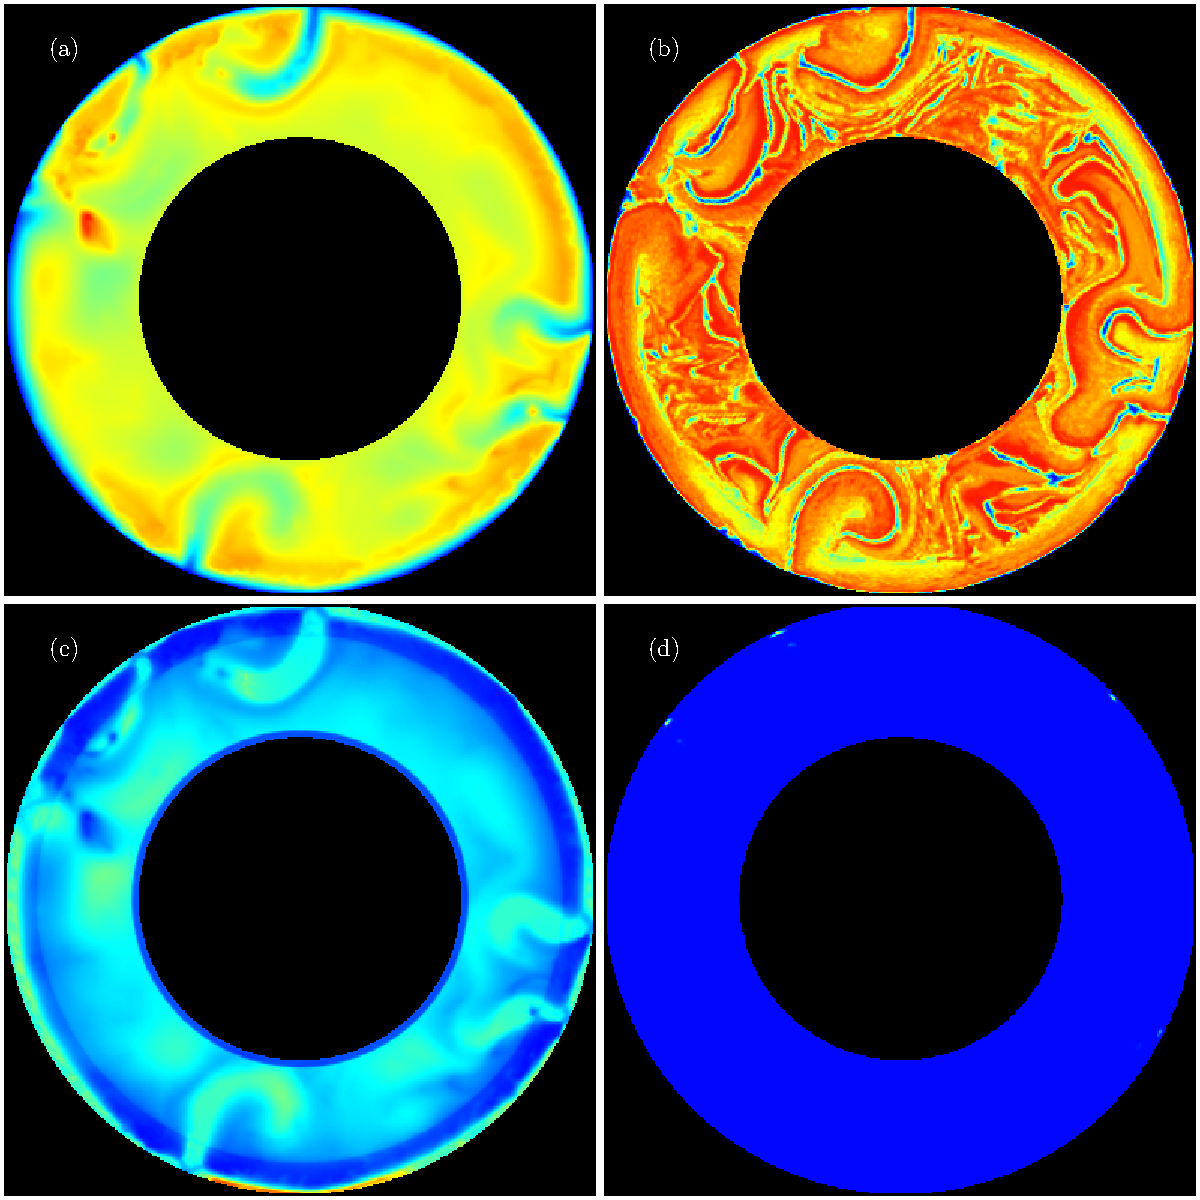
\includegraphics[width=\linewidth]{1-050-1_327_grid.pdf}
\caption{The end result of running a 1 $M_\odot$ model with a yield stress of 50 Mpa and internal heating rate of 5.2 $\times 10^{-12}$ W/kg for 10 billion years. Panels (a)--(d) represent fields of temperature, composition, viscosity, and melt fraction, respectively. Plate tectonics are evident in this regime, as is clear from the subduction zones visible throughout these figures.}
\label{fig:M1Q1Y1}
\end{figure}

\begin{figure}
\centering
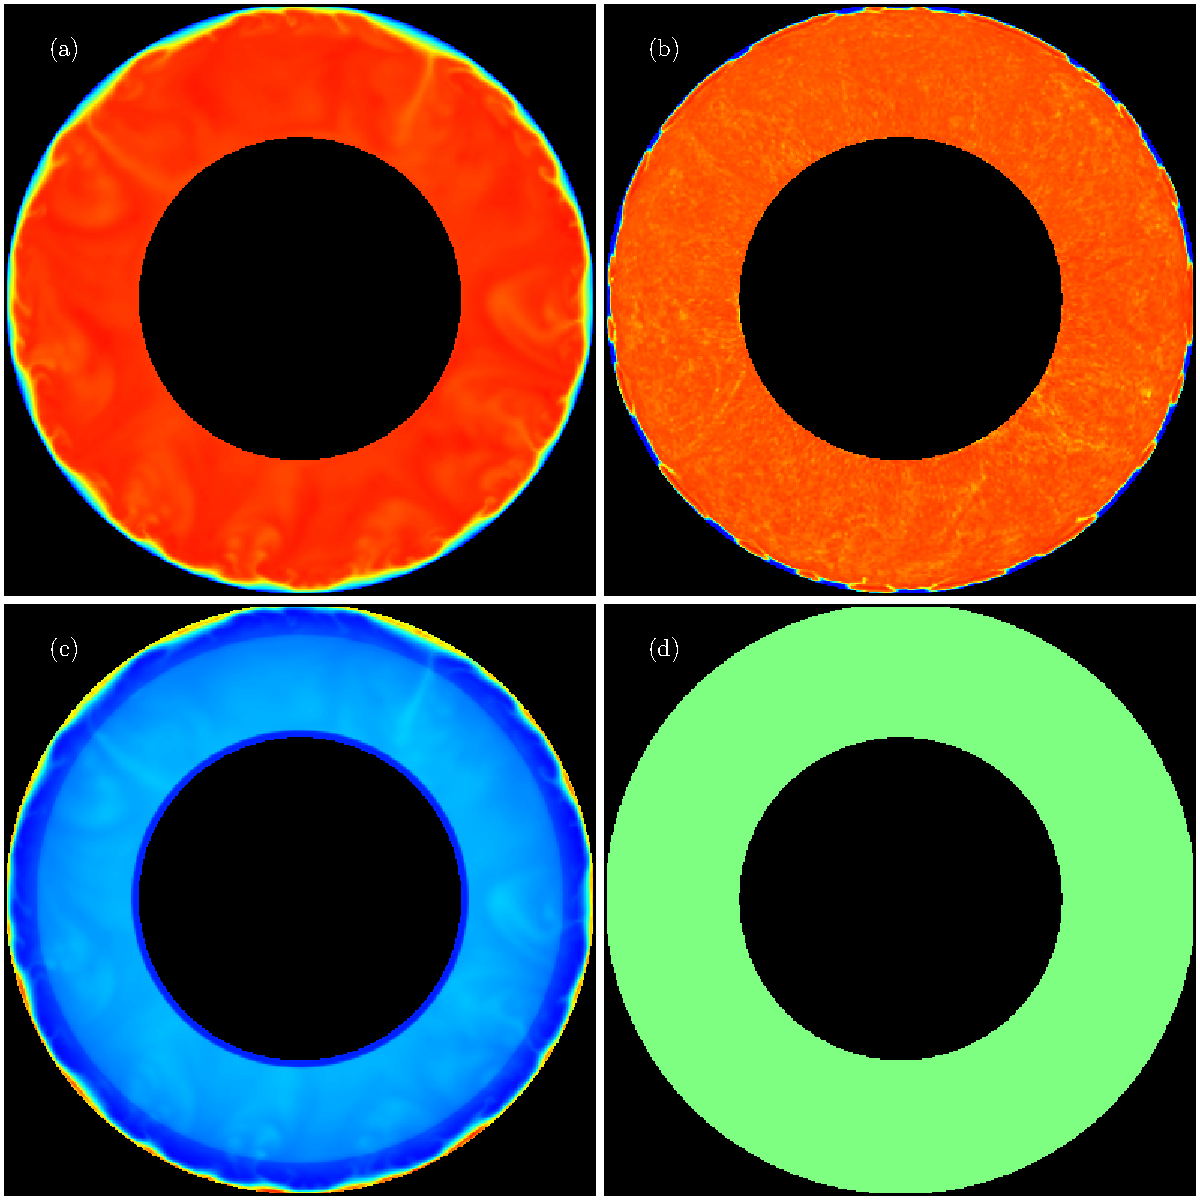
\includegraphics[width=\linewidth]{1-250-1_293_grid.pdf}
\caption{The end result of running a 1 $M_\odot$ model with a yield stress of 250 Mpa and internal heating rate of 5.2 $\times 10^{-12}$ W/kg for 10 billion years. Panels (a)--(d) are as described in the caption of Fig. \ref{fig:M1Q1Y1}. This model demonstrates a stagnant lid (i.e. single plate) regime.}
\label{fig:M1Q1Y5}
\end{figure}

\begin{figure*}
\centering
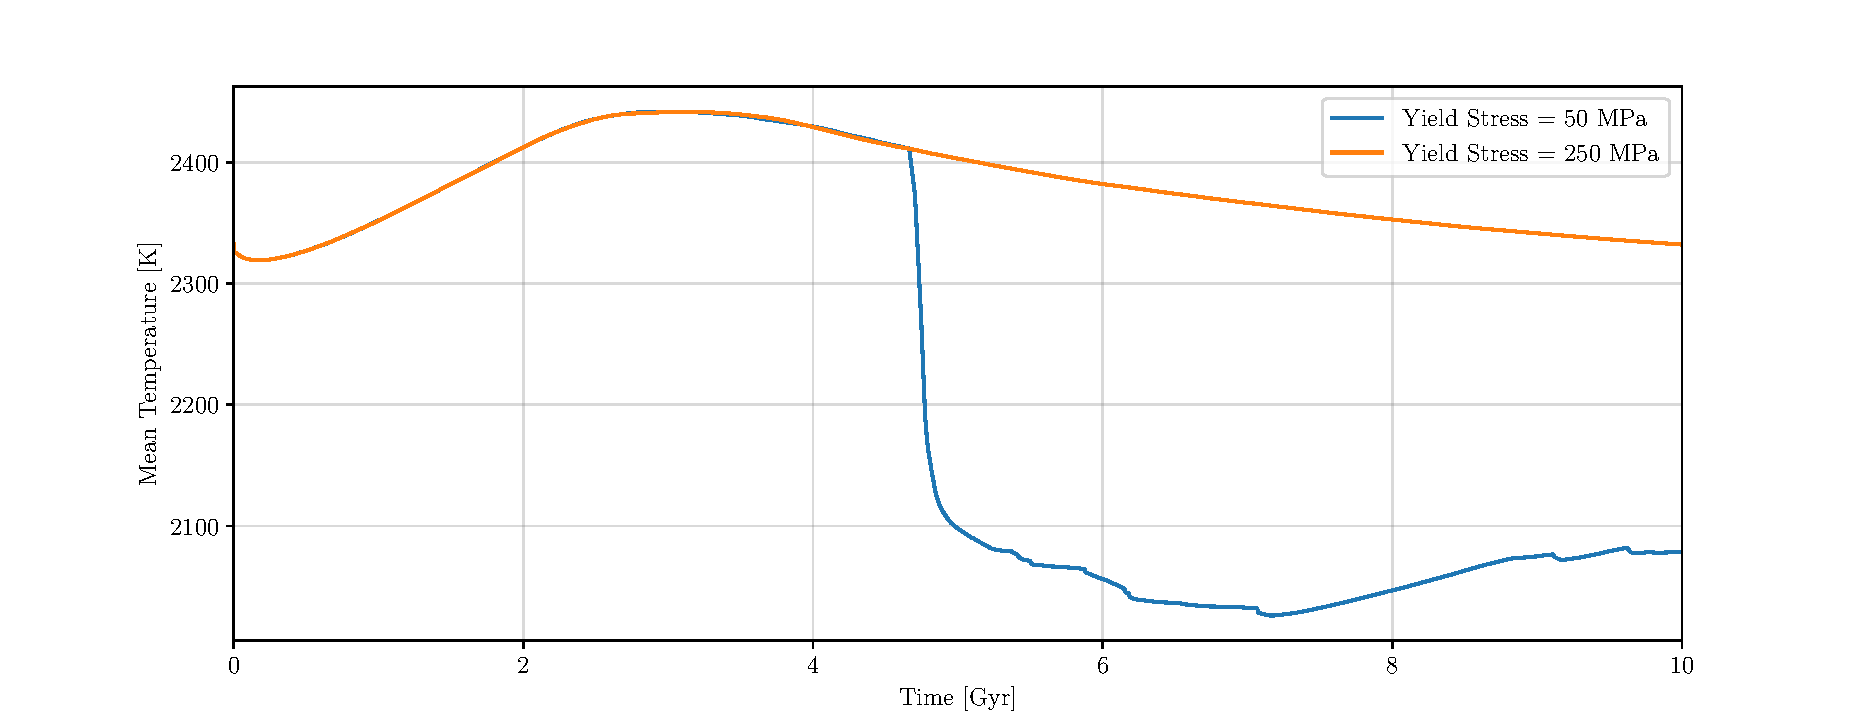
\includegraphics[width=\textwidth]{M1Q1Y1-5_T.pdf}
\caption{The change in temperature over time of 1  $M_\odot$ models with yield stresses of 50 and 250 Mpa and internal heating rates of 5.2 $\times 10^{-12}$ W/kg. In the model with a yield stress of 50 MPa, the transition to plate tectonics is visible at $\sim$ 4.6 Gyr, where the temperature drops steeply. Following this, the temperature varies slightly but eventually seems to settle into a quasi-steady state. In the 250 MPa yield stress model, the planet is in a stagnant lid regime and the interior slowly cools over time. These results should be compared with the fields displayed in Figs. \ref{fig:M1Q1Y1} and \ref{fig:M1Q1Y5}.}
\label{fig:M1Q1Y1-5_temperature}
\end{figure*}

\section{Discussion} \label{sec:discussion}
\section{Conclusion} \label{sec:conc}

\begin{thebibliography}{}
\bibitem[Barclay et al.(2018)]{Barclay18} Barclay, T., Pepper, J., \& Quintana, E. V. 2018, arXiv preprint
\bibitem[Barnes et al.(2008)]{Barnes08} Barnes, R., Raymond, S. N., Jackson, B., \& Greenberg, R. 2008, AsBio, 8, 557
\bibitem[Barnes et al.(2013)]{Barnes13} Barnes, R., Mullins, K., Goldblatt, C. et al. 2013, AsBio, 13, 225
\bibitem[Crouzet et al.(2017)]{Crouzet17} Crouzet, N., Bonfils, X., Delfosse, X., et al. 2017, arXiv preprint
\bibitem[Foley \& Smye(2018)]{Foley18} Foley, B. J. \& Smye, A. J. 2018, AsBio, 18, 7
\bibitem[Gando et al.(2011)]{Gando11} Gando, A., Gando, Y., Ichimura, K., et al. 2011, Nature GeoScience, 4, 647
\bibitem[Jackson et al.(2008b)]{Jackson08b} Jackson, B., Barnes, R., \& Greenberg, R. 2008, MNRAS, 391, 237
\bibitem[Kasting et al.(1993)]{Kasting93} Kasting, J. F., Whitmire, D. P., \& Reynolds, R. T. 1993, Icarus, 101, 108
\bibitem[Kite et al.(2011)]{Kite11} Kite, E. S., Gaidos, E., \& Manga, M. 2011, \apj, 743, 41
\bibitem[Korenaga(2012)]{Korenaga12} Korenaga, J. 2012, \textit{Ann. N.Y. Acad. Sci.}, 1260, 87
\bibitem[Louie et al.(2018)]{Louie18} Louie, D. R., Deming, D., Albert, L., et al. 2018, PASP, 130, 440
\bibitem[Makarov et al.(2018)]{Makarov18} Makarov, V. V., Berghea, C. T., \& Efroimsky, M. 2018, \apj, 857, 142
\bibitem[Moresi \& Solomatov(1998)]{Moresi98} Moresi, L. \& Solomatov, V. 1998, \textit{Geophys. J. Int.}, 133(3), 669
\bibitem[Petrovich et al.(2018)]{Petrovich18} Petrovich, C., Deibert, E., \& Wu, Y. 2018, arXiv preprint
\bibitem[Rowley et al.(2016)]{Rowley16} Rowley, D. B., Forte, A. M., Rowan, C. J., et al. 2016, Science Advances, 2, 12
\bibitem[Stern et al.(2018)]{Stern18} Stern, R. J., Gerya, T., \& Tackley, P. J 2018, \textit{Geoscience Frontiers}, 9, 103
\bibitem[Tackley(2000)]{Tackley00} Tackley, P. J. 2000, \textit{Geochem., Geophys., Geosys.}, 1, 1
\bibitem[Tackley et al.(2008)]{Tackley08} Tackley, P. J. 2008, PEPI, 171, 7
\bibitem[Tackley(2013)]{Tackley13} Tackley, P. J. 2013, \texttt{StagYY} User Guide
\bibitem[Tackley et al.(2014)]{Tackley14} Tackley, P. J., Ammann, M. M., Brodholt, J. P., et al. 2014, \textit{IAUS}, 293, 339
\bibitem[Turcotte(1993)]{Turcotte93} Turcotte, D. L. 1993, \textit{Journal of Geophysical Research}, 98, E9
\bibitem[Turcotte \& Schubert(2002)]{Turcotte02} Turcotte, D. \& Schubert, G. 2002, \textit{Geodynamics}
\bibitem[Williams \& Kasting(1997)]{Williams97} Williams, D. M. \& Kasting, J. F. 1997, \textit{Icarus}, 129, 254
\bibitem[Zhong et al.(2007)]{Zhong07} Zhong, S., Yuen, D. A., \& Moresi, L. N. 2007, Elsevier, 7
\end{thebibliography}

\end{document}
